\scanpage{200}
% archive sheet number: 199

\handwritten{\diagram{\begin{tikzcd}[ampersand replacement=\&,row sep=small,column sep=small]
 A\arrow[rr,Rightarrow] \& \& B\\
 A^{\unsure{\mathfrak S|\mathscr S}_3^+}\arrow[u,"3"]\arrow[rr,dash,"2"] \& \& B_1=B^{\mathfrak S_3^+}\arrow[u,dash,"3"']\\
 \& B^{\mathfrak S_3}\arrow[ur,dash] \& \\
 A^{\mathfrak S_3}\arrow[uu,"2"]\arrow[ur,dash]\arrow[rr,dash,"2"] \& \& B_{\unsure{0|\circ}}\arrow[uu,dash,"2"']
\end{tikzcd}}}

\handwritten{\[
 \begin{aligned}
 &\alpha+\beta\tau+\alpha'+\beta'\tau'\\
 &=(\alpha+\alpha')+\bigl(\beta\tau+\beta'(\sigma-\tau)\bigr)\\
 &=\underline{\alpha+\alpha'}+\underline{\beta'\sigma}+(\beta-\beta')\tau
 \end{aligned}
\]}

\handwritten{\[
 \alpha+\alpha'+\beta\sigma-(\alpha+\alpha'+\beta'\sigma)=(\beta-\beta')\sigma\qquad\mathrm{OK}
\]}

% Typed passage runs sideways relative to the handwritten calculations.
\mspage{L 22}

% Black shape touching the j; shown in the reading direction of the type.
\figure{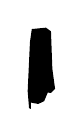
\begin{tikzpicture}[x=.58cm,y=.58cm]
\fill (0,0)--(-.03,.37)--(.02,1.45)--(.06,1.73)--(.37,1.76)--(.48,1.68)--(.51,.86)--(.57,.42)--(.48,.33)--(.41,.34)--(.33,.15)--(.20,.09)--(.04,.12)--(.04,-.02)--cycle;
\end{tikzpicture}}

Tout ce que \unsure{je} croyais avoir à dire, à un moment ou à un autre\deleted{\unsure{s|d}} de la réflexion, \handwritten{(}que ce soit sur moi, ou sur tel autre, ou sur un milieu, ou sur une époque, je l'ai dit, sans \inserted{jamais} avoir à bousculer mes réticences. Il a suffi à chaque fois que je les examine avec attention, pour qu'elles s'évanouissent\deleted{\unsure{,|.}} sans plus laisser de traces.
